\chapter{Vulnerabilità implementazioni DDS}
\label{chvulimpldds}

In questo capitolo verranno mostrati dei casi studio
di tre tipologie di 
attacco che vengono effettuati tramite delle 
implementazioni del DDS dei vari vendors.

L'obiettivo di questi casi studio è di trovare delle 
vulnerabilità in Robot Operating System (ROS) 2 che 
utilizza come middleware il DDS e come wire-protocol 
l'RTPS (Real-Time Publish-Subscribe Protocol).
Infatti saranno proprio i pacchetti RTPS a contenere 
l'exploit vero e proprio. Prima di mandare questi 
pacchetti è stato necessario creare una libreria Python 
così da poter automatizzare il loro processo di creazione.
Questo strumento, successivamente è stato anche unito al 
progetto Scapy di Python, nella 
Figura~\ref{rptspacketheaderscapy} è presente un esempio 
di un pacchetto RTPS costruito con questa libreria.

\begin{figure}[H]
    \centering
    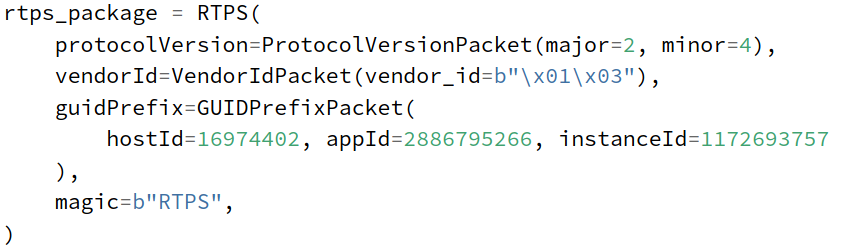
\includegraphics[width=15.2cm, keepaspectratio]{img/rptspacketheaderscapy.png}
    \caption{Un pacchetto RTPS costruito 
    con Scapy \cite{mayoral2022robot}.}
    \label{rptspacketheaderscapy}
\end{figure}

\section{Ricognizione DDS}
Le implementazioni DDS, per rispettare lo standard 
OMG, devono seguire delle regole di interoperabilità 
per far si che i vari applicativi DDS siano compatibili 
tra di loro. Questo ha portato alla creazione di un sistema
molto verbose per effettuare discovery 
di altri partecipanti all'interno di un network DDS.


La natura molto verbose del processo di autoscoperta 
fa si che inviando un singolo pacchetto RTPS vuoto 
a un'entità di una rete DDS all'interno di un dominio,
quest'ultima risponderà 
con un messaggio discovery. La risposta, mostrata
in Figura~\ref{rispostarecoinnassance} ci permetterà di 
confermare se quel determinato partecipante è attivo.

\begin{figure}[H]
    \centering
    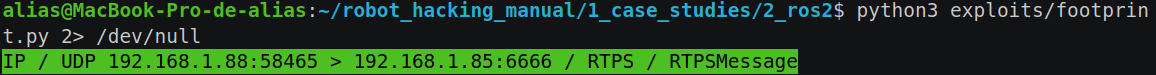
\includegraphics[width=15.2cm, keepaspectratio]{img/rispostarecoinnassance.png}
    \caption{Esempio di risposta discovery di un'entità DDS
    \cite{mayoral2022robot}.}
    \label{rispostarecoinnassance}
\end{figure}

La vulnerabilità è stata individuata adoperando 
CycloneDDS, ma anche altre implementazioni 
presentano lo stesso problema. 
Questo accade perché non è possibile mitigare 
la vulnerabilità senza violare lo standard 
OMG. L'unica soluzione applicabile consisterebbe 
nel disabilitare in parte il meccanismo di autoscoperta, 
ma cosi facendo l'interoperabilità tra i vari vendors 
DDS andrebbe persa. 

Per questo motivo, dato che i vendors 
preferiscono mantenere questa interoperabilità non esiste 
una soluzione vera e propria \cite{mayoral2022robot}.


\section{Attacco riflesso DDS}
Un attacco riflesso consiste nel dirottare il traffico 
di rete verso un dispositivo vittima, manipolando e in certi 
casi amplificando anche un flusso di dati.

\begin{figure}[H]
    \centering
    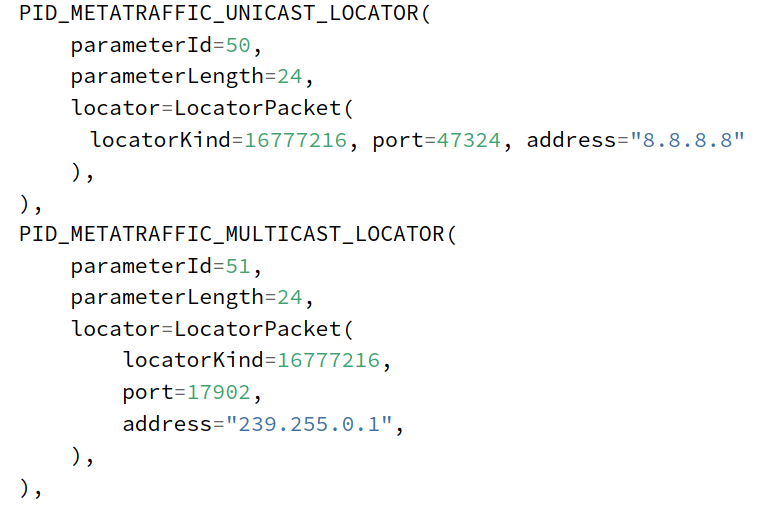
\includegraphics[width=15.2cm, keepaspectratio]{img/submessaggereflection.png}
    \caption{Parte di un pacchetto RTPS costruito con Scapy
    che abilita un attacco
    riflesso \cite{mayoral2022robot}.}
    \label{submessaggereflection}
\end{figure}

Il vettore di questo attacco si trova all'interno di più parametri 
di un sottomessaggio di tipo DATA 
incluso il parametro 
\texttt{PID\_METATRAFFIC\_MULTICAST\_LOCATOR} che si occupa di specificare 
gli indirizzi multicast che verranno adoperati successivamente dalle 
entità per comunicazioni di metatraffico.
Il DDS non prevede filtri per questo 
specifico valore e quindi un attaccante può specificare a un 
partecipante di utilizzare un indirizzo IP multicast per il metatraffico 
sotto il suo controllo. Ricevuto questo traffico l'attaccante può 
ricevere informazioni riguardo la rete DDS e rispondere al partecipante
con un alto numero di comunicazioni in modo tale da sovraccaricarlo (DDoS).

Inoltre, il valore 
di \texttt{PID\_METATRAFFIC\_MULTICAST\_LOCATOR} può essere utilizzato 
da un attore malevolo per reindirizzare il traffico di molteplici 
entità verso un unico partecipante che si ritoverà quindi a ricevere un 
numero elevato di pacchetti indesiderati rallentandone la sua esecuzione.

Un altro parametro simile è il \texttt{PID\_METATRAFFIC\_UNICAST\_LOCATOR}
che si occupa di specificare un indirizzo IP di tipo unicast 
per la comunicazioni di metatraffico. Anche in questo caso non è
possibile applicare filtri per limitare la scelta di valori per 
gli indirizzi IP. 

Come mostrato nella 
Figura~\ref{submessaggereflection} creando un pacchetto con Scapy e
modificando i valori dei parametri vulnerabili 
sarà possibile 
rispedire le comunicazioni di una identità verso un qualsiasi
indirizzo, come l'IP del DNS 8.8.8.8 (Figura~\ref{reflectionattackdns}).


\begin{figure}[H]
    \centering
    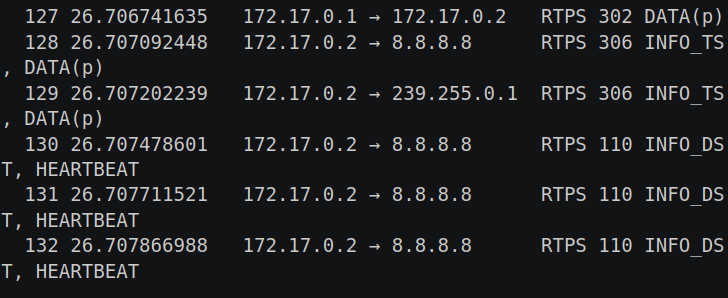
\includegraphics[width=15.2cm, keepaspectratio]{img/reflectionattackdns.png}
    \caption{Esempio di reindirizzamento dei messaggi verso il server DNS 8.8.8.8
    \cite{mayoral2022robot}.}
    \label{reflectionattackdns}
\end{figure}

Questo problema di sicurezza è presente in tutte le implementazioni,
come viene mostrato dai CVE della Figura~\ref{CVErecoinnassance},
dei vendor dato che non può essere risolto senza violare lo 
standard OMG. Questa opzione però, non è considerata dai vari 
vendors perché interromperebbe l'interoperabilità tra le 
diverse implementazioni.
Per rimanere compatibili con lo standard OMG i vendor hanno 
implementato un sistema di controllo che limita il numero 
di pacchetti scambiati quando viene superata una soglia limite
prefissata. Questo sistema non è perfetto, ma in molti casi ha 
ridotto significativamente 
l'efficacia di questo attacco \cite{mayoral2022robot}.

\begin{figure}[H]
    \centering
    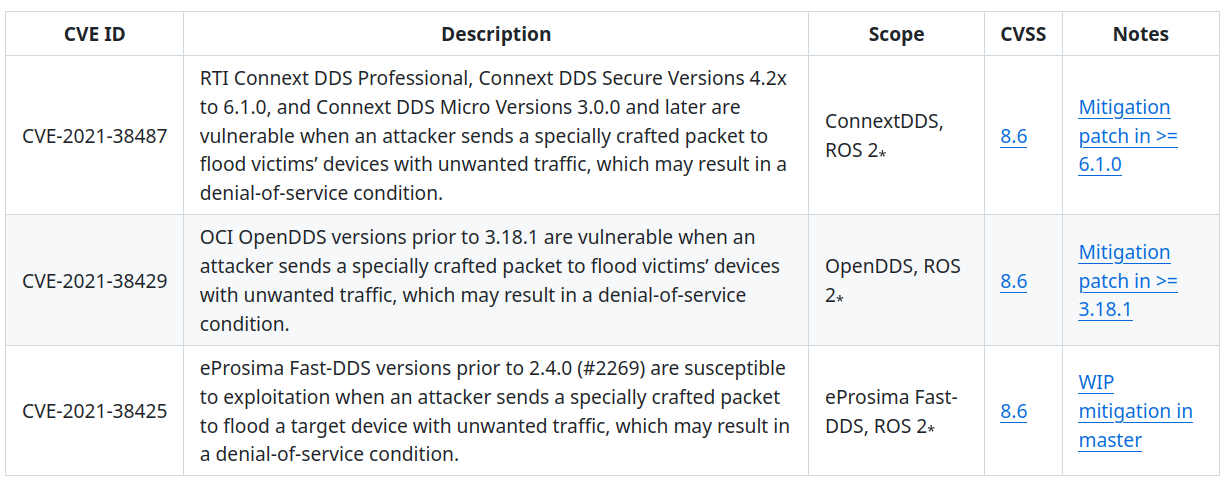
\includegraphics[width=15.2cm, keepaspectratio]{img/CVErecoinnassance.png}
    \caption{Varie CVE per attacco riflesso \cite{mayoral2022robot}.}
    \label{CVErecoinnassance}
\end{figure}


\section{Crash di un partecipante}
La seguente vulnerabilità è stata scoperta utilizzando 
un software in grado di eseguire fuzz tests, 
incluso DDSFuzz (mostrato nella Sezione~\ref{ddsfuzz}).

I test hanno identificato una vulnerabilità in un mancato 
controllo di lunghezza del valore del parametro 
\texttt{PID\_BUILTIN\_ENDPOINT\_QOS} che si trova all'interno di 
un sottomessaggio utilizzato durante la fase di autoscoperta
del DDS \cite{mayoral2022robot}. 

Questo parametro viene 
utilizzato nella fase di discovery
tra i partecipanti della rete per trasmettere
alla nuova entità, che vuole unirsi alla rete, le policy
QoS attive. La nuova entità, confrontate 
le proprie impostazioni QoS con quelle appena ricevute
può determinare con quali partecipanti può iniziare le 
comunicazioni \cite{ddsrtps}.

Data la mancanza di un controllo per la lunghezza del 
valore del parametro è possibile costruire un pacchetto 
RTPS, come mostrato in Figura~\ref{crashnode} 
in modo tale da 
mandare in crash il partecipante che lo riceve. 
Osserviamo che il valore \texttt{parameterLength} è pari a zero,
mentre il parametro \texttt{parameterData} contiene dei bytes 
(nel nostro caso nulli).
Questa discrepanza causa un crash durante la 
lettura di \texttt{parameterData} dato che l'indice di lettura 
venendo impostato (\texttt{parameterLength}) a zero 
denota che non dovrebbe essere 
presente alcun dato al suo interno. 
Di conseguenza,
viene eseguita una porzione di codice al di fuori dei 
limiti della memoria causando un errore di segmentazione.

Inoltre, 
non viene esclusa la possibilità che questa vulnerabilità 
possa essere sfruttata per eseguire del codice arbitrario 
malevolo.

\begin{figure}[H]
    \centering
    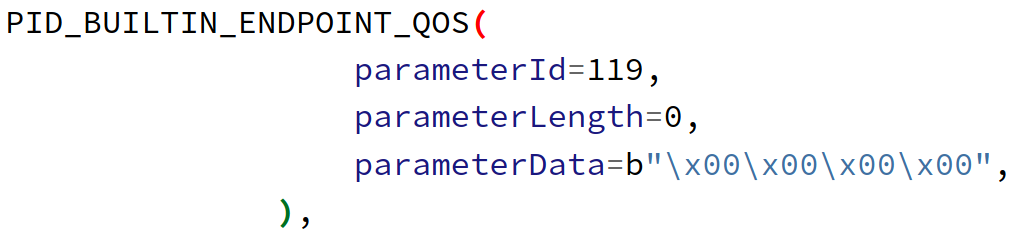
\includegraphics[width=15.2cm, keepaspectratio]{img/crashnode.png}
    \caption{Pacchetto RTPS con il valore di parameterLength incorretto 
    \cite{mayoral2022robot}.}
    \label{crashnode}
\end{figure}


Questa vulnerabilità è stata individuata solamente 
nell'implementazione Fast DDS.
Successivamente 
è stata registrata una segnalazione CVE, mostrata in 
Figura~\ref{CVEnodecrashing},
che ha portato 
al rilascio di una patch per correggere il problema \cite{mayoral2022robot}.


\begin{figure}[H]
    \centering
    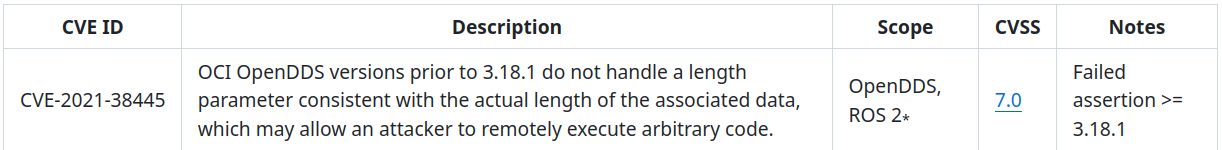
\includegraphics[width=15.2cm, keepaspectratio]{img/CVE node crashing.png}
    \caption{CVE per mancato controllo di lunghezza 
    di \texttt{PID\_BUILTIN\_ENDPOINT\_QOS} \cite{mayoral2022robot}.}
    \label{CVEnodecrashing}
\end{figure}
